% !TeX program = xelatex
\documentclass[a4paper,10pt]{article}

% ============================================================================
% កញ្ចប់សម្ភារៈសិក្សាបោះពុម្ព ស-ខ្មៅ (Printable Classroom Materials - Grade 8 RAT23)
% ត្រូវគ្នា ១០០% នឹង LS_Plan_RAT23.tex និង Teaching_Scenario_RAT23.tex
% ============================================================================
\usepackage[a4paper, left=1.0cm, right=1.0cm, top=0.75cm, bottom=1.05cm, footskip=0.55cm]{geometry}
\usepackage{amsmath, amssymb}
\usepackage{unicode-math}
\usepackage{fontspec}
\usepackage{array, colortbl}
\usepackage[table]{xcolor}
\usepackage{enumitem}
\usepackage{pifont}
\usepackage{fancyhdr}
\usepackage{lastpage}
\usepackage{tikz}
\usepackage[most]{tcolorbox}
\usetikzlibrary{calc, arrows.meta, decorations.markings, positioning, babel}

% LaTeX 2025 compatibility guard
\makeatletter
\let\@expl@@@mark@update@singlecol@structures@@\relax
\makeatother

% ============================================================================
% ការកំណត់ពុម្ពអក្សរផ្លូវការ (Cross-Platform Windows + Cloud fonts/)
% ============================================================================
\providecommand{\NGSFindFonts}{%
  \IfFileExists{C:/Windows/Fonts/cambria.ttc}{%
    \def\NGSSysPath{C:/Windows/Fonts/}%
    \def\NGSUserPath{C:/Users/KIT/AppData/Local/Microsoft/Windows/Fonts/}%
  }{%
    \IfFileExists{./fonts/KhmerOSsiemreap.ttf}{\def\NGSSysPath{./fonts/}\def\NGSUserPath{./fonts/}}{%
    \IfFileExists{../fonts/KhmerOSsiemreap.ttf}{\def\NGSSysPath{../fonts/}\def\NGSUserPath{../fonts/}}{%
    \IfFileExists{../../fonts/KhmerOSsiemreap.ttf}{\def\NGSSysPath{../../fonts/}\def\NGSUserPath{../../fonts/}}{%
    \IfFileExists{../../../fonts/KhmerOSsiemreap.ttf}{\def\NGSSysPath{../../../fonts/}\def\NGSUserPath{../../../fonts/}}{%
    \IfFileExists{../../../../fonts/KhmerOSsiemreap.ttf}{\def\NGSSysPath{../../../../fonts/}\def\NGSUserPath{../../../../fonts/}}{%
    \IfFileExists{../../../../../fonts/KhmerOSsiemreap.ttf}{\def\NGSSysPath{../../../../../fonts/}\def\NGSUserPath{../../../../../fonts/}}{%
    \IfFileExists{../../../../../../fonts/KhmerOSsiemreap.ttf}{\def\NGSSysPath{../../../../../../fonts/}\def\NGSUserPath{../../../../../../fonts/}}{%
      \def\NGSSysPath{../../../../../../../fonts/}\def\NGSUserPath{../../../../../../../fonts/}%
    }}}}}}}%
  }%
}
\NGSFindFonts

\setmathfont[
  Path={\NGSSysPath},
  FontIndex=1,
  Scale=1.02
]{cambria.ttc}

\defaultfontfeatures{Ligatures=TeX}

\setmainfont[
  Path={\NGSUserPath},
  Extension=.ttf,
  Script=Khmer,
  BoldFont={KhmerOSsiemreap},
  BoldFeatures={FakeBold=1.8},
  ItalicFont={KhmerOSsiemreap},
  ItalicFeatures={FakeSlant=0.25},
  BoldItalicFont={KhmerOSsiemreap},
  BoldItalicFeatures={FakeBold=1.8, FakeSlant=0.25}
]{KhmerOSsiemreap}

\newfontfamily\muol[
  Path={\NGSUserPath},
  Extension=.ttf,
  Script=Khmer
]{KhmerOSmuollight}

\newfontfamily\TimesEn[
  Path={\NGSSysPath},
  Extension=.ttf,
  BoldFont={timesbd},
  ItalicFont={timesi},
  BoldItalicFont={timesbi}
]{times}

\newfontfamily\CalibriFont[
  Path={\NGSSysPath},
  Extension=.ttf
]{calibri}

\newfontfamily\Tacteing[
  Path={\NGSUserPath}
]{TACTENG.TTF}

\XeTeXlinebreaklocale "km"
\XeTeXlinebreakskip = 0pt plus 1pt minus 0.1pt

% ============================================================================
% ក្ដារពណ៌ ស-ខ្មៅ សុទ្ធសម្រាប់ការបោះពុម្ព (Strict Monochrome Print Palette)
% ============================================================================
\definecolor{panelgray}{gray}{0.93}
\definecolor{headgray}{gray}{0.86}
\definecolor{midgray}{gray}{0.76}
\definecolor{darkline}{gray}{0.35}

\pagestyle{fancy}
\fancyhf{}
\renewcommand{\headrulewidth}{0pt}
\fancyfoot[L]{\fontsize{8.0pt}{10.5pt}\selectfont អនុវិទ្យាល័យព្រះក្រសាំង \en{---} គណិតវិទ្យា ថ្នាក់ទី៨ \en{|} មេរៀនទី១ (២.៣) លក្ខណៈនៃចំនួនសនិទាន (ស-ខ្មៅ) \en{|} ថ្ងៃចន្ទ ៧កើត កត្តិក ២៥៧០ \en{|} ១៦ វិច្ឆិកា ២០២៦}
\fancyfoot[R]{\fontsize{8.4pt}{10.5pt}\selectfont ទំព័រ \en{\thepage\ / \pageref{LastPage}}}

\setlength{\parindent}{0pt}
\setlength{\parskip}{0pt}
\setlength{\tabcolsep}{4pt}

% ============================================================================
% ម៉ាក្រូជំនួយ (Helper Macros)
% ============================================================================
\newcommand{\en}[1]{{\TimesEn #1}}
\newcommand{\enbf}[1]{{\TimesEn\bfseries #1}}
\newcommand{\unit}[1]{\,\text{\en{#1}}}
\newcommand{\cnum}[1]{\mbox{\TimesEn\fontsize{10pt}{12pt}\selectfont\ding{\numexpr181+#1\relax}}}
\newcommand{\scissors}{\ding{34}}
\newcommand{\chkbox}{\tikz[baseline=-0.15ex]\draw[black, line width=0.9pt] (0,0) rectangle (0.26cm,0.26cm);}
\newcommand{\khmflourish}{{\Tacteing\fontsize{32pt}{13pt}\selectfont\raisebox{-4pt}{3}}}

\newcommand{\pagebanner}[2]{%
  \begin{tcolorbox}[
    enhanced, sharp corners, colback=headgray, colframe=black,
    boxrule=1.1pt, boxsep=1.5pt, top=3.5pt, bottom=3.5pt, left=6pt, right=6pt,
    after skip=5pt
  ]
    {\muol\fontsize{9.5pt}{14pt}\selectfont #1}\hfill{\fontsize{8.5pt}{12pt}\selectfont\textbf{#2}}
  \end{tcolorbox}%
}

\newcolumntype{L}[1]{>{\raggedright\arraybackslash}p{#1}}
\newcolumntype{C}[1]{>{\centering\arraybackslash}p{#1}}

\begin{document}
\fontsize{9.5pt}{14.0pt}\selectfont

% ============================================================================
% ទំព័រទី ១៖ សម្ភារៈ E2 ខ្នាតពិត 1:1 (បន្ទះប្រភាគសមមូល 7.00 cm + បន្ទាត់ចំនួនឆ្លុះ 12.00 cm)
% ============================================================================
\pagebanner{សម្ភារៈទី ១៖ បន្ទះកាត់ \enbf{E2} ខ្នាតពិត \enbf{1:1} ប្រភាគសមមូល \enbf{\&} បន្ទាត់ចំនួនឆ្លុះ \enbf{POE 2A--2B}}{ទំព័រ ១/៦ \en{-- E2 Explore}}

\noindent
\begin{minipage}[c]{11.7cm}
  \begin{tcolorbox}[
    enhanced, sharp corners, colback=panelgray, colframe=black,
    boxrule=1.0pt, boxsep=1.5pt, top=3.5pt, bottom=3.5pt, left=6pt, right=6pt
  ]
    \fontsize{8.8pt}{12.8pt}\selectfont
    \textbf{ការណែនាំសំខាន់មុនបោះពុម្ព (\en{Print at 100\% / Actual Size})៖} ត្រូវជ្រើស \textbf{\en{Scale: Actual Size 100\%}} (\textbf{ហាមជ្រើស \en{Fit to Page}}) ដើម្បីឱ្យបន្ទះប្រភាគគោល $7.00\unit{cm}$ ($\frac{5}{7}=5.00\unit{cm}$) និងបន្ទាត់ចំនួនឆ្លុះ ($1\text{ ឯកតា}=6.00\unit{cm}$) ត្រូវខ្នាតពិត \en{1:1} ឥតល្អៀង។
  \end{tcolorbox}
\end{minipage}%
\hfill
\begin{minipage}[c]{7.0cm}
  \begin{tcolorbox}[
    enhanced, sharp corners, colback=white, colframe=black,
    boxrule=1.0pt, boxsep=1pt, top=3pt, bottom=3pt, left=4pt, right=4pt
  ]
    \centering
    {\fontsize{8.2pt}{10.5pt}\selectfont\textbf{បន្ទះផ្ទៀងខ្នាតពិត \en{5.00 cm} (\en{Actual Size 100\%})}}\\[2pt]
    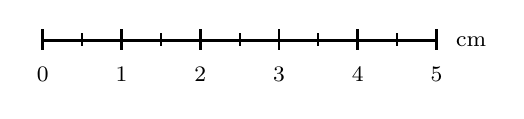
\begin{tikzpicture}[x=1cm, y=1cm, every node/.style={font=\footnotesize, text=black}]
      \draw[black, line width=1.1pt] (0,0) -- (5,0);
      \foreach \x in {0,1,2,3,4,5} {
        \draw[black, line width=1.0pt] (\x,-0.12) -- (\x,0.14);
        \node[below=2.5pt] at (\x,-0.12) {\en{\x}};
      }
      \foreach \m in {0.5,1.5,2.5,3.5,4.5} {
        \draw[black, line width=0.8pt] (\m,-0.07) -- (\m,0.09);
      }
      \node[right=3pt] at (5.02,-0.02) {\en{cm}};
    \end{tikzpicture}
  \end{tcolorbox}
\end{minipage}

\vspace{5pt}

% --- ប្រអប់កាត់ទី១៖ បន្ទះប្រភាគសមមូល 1:1 (x=1cm, y=1cm គ្មានការបង្រួម) ---
\begin{tcolorbox}[
  enhanced, sharp corners, colback=white, colframe=black,
  boxrule=1.0pt, borderline={0.8pt}{2pt}{black, dashed},
  top=5pt, bottom=5pt, left=7pt, right=7pt
]
  {\textbf{\scissors\ ផ្នែកកាត់ទី១ — បន្ទះប្រភាគសមមូលខ្នាតពិត \en{1:1} (បន្ទះគោល $1\text{ ឯកតា} = 7.00\unit{cm}$)}៖ កាត់ ឬវាស់ផ្ទៀងដោយបន្ទាត់ \en{cm}}\\[4pt]
  \begin{center}
  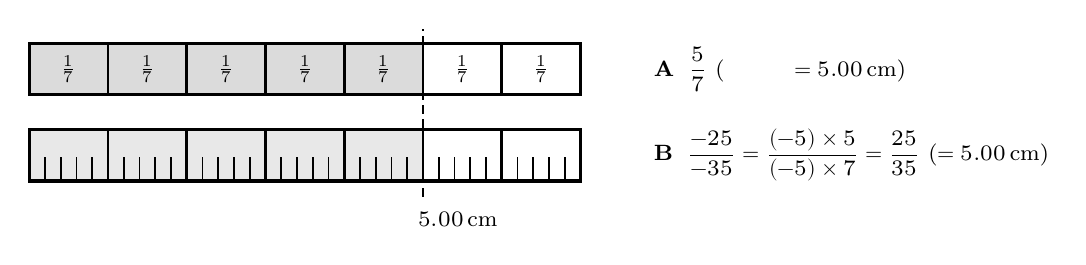
\begin{tikzpicture}[x=1cm, y=1cm, every node/.style={font=\footnotesize, text=black}]
    % បន្ទះ A: 5/7 (5.00 cm នៃ 7.00 cm)
    \fill[gray!28] (0,1.25) rectangle (5.00,1.90);
    \draw[black, line width=1.15pt] (0,1.25) rectangle (7.00,1.90);
    \foreach \k in {1,...,6} {
      \draw[black, line width=0.95pt] (\k,1.25) -- (\k,1.90);
    }
    \foreach \k in {1,...,7} {
      \node at ({\k-0.5},1.57) {$\frac{1}{7}$};
    }
    \node[anchor=west] at (7.30,1.57) {\textbf{បន្ទះ \en{A}៖} $\dfrac{5}{7}$ (ប្រវែងផាត់ $= 5.00\unit{cm}$)};

    % បន្ទះ B: 25/35 = -25/-35 (25 x 0.20 cm = 5.00 cm នៃ 7.00 cm)
    \fill[gray!18] (0,0.15) rectangle (5.00,0.80);
    \draw[black, line width=1.15pt] (0,0.15) rectangle (7.00,0.80);
    \foreach \k in {1,...,6} {
      \draw[black, line width=1.0pt] (\k,0.15) -- (\k,0.80);
    }
    \foreach \m in {1,...,34} {
      \draw[black, line width=0.65pt] ({0.20*\m},0.15) -- ({0.20*\m},0.46);
    }
    \draw[black, densely dashed, line width=1.0pt] (5.00,-0.05) -- (5.00,2.08);
    \node[below=2pt] at (5.00,-0.05) {គំនូសផ្ទឹម $5.00\unit{cm}$};
    \node[anchor=west] at (7.30,0.48) {\textbf{បន្ទះ \en{B}៖} $\dfrac{-25}{-35}=\dfrac{(-5)\times 5}{(-5)\times 7}=\dfrac{25}{35}$ ($=5.00\unit{cm}$)};
  \end{tikzpicture}
  \end{center}
\end{tcolorbox}

\vspace{5pt}

% --- ប្រអប់កាត់ទី២៖ បន្ទាត់ចំនួនឆ្លុះគល់ 0 ខ្នាតពិត 1:1 (1 unit = 6.00 cm, [-1,+1] = 12.00 cm) ---
\begin{tcolorbox}[
  enhanced, sharp corners, colback=white, colframe=black,
  boxrule=1.0pt, borderline={0.8pt}{2pt}{black, dashed},
  top=5pt, bottom=5pt, left=7pt, right=7pt
]
  {\textbf{\scissors\ ផ្នែកកាត់ទី២ — បន្ទាត់ចំនួនឆ្លុះគល់ $0$ ខ្នាតពិត \en{1:1} ($1\text{ ឯកតា} = 6.00\unit{cm}$)}៖ បត់តាមបន្ទាត់ដាច់ៗត្រង់គល់ $0$!}\\[3pt]
  \begin{center}
  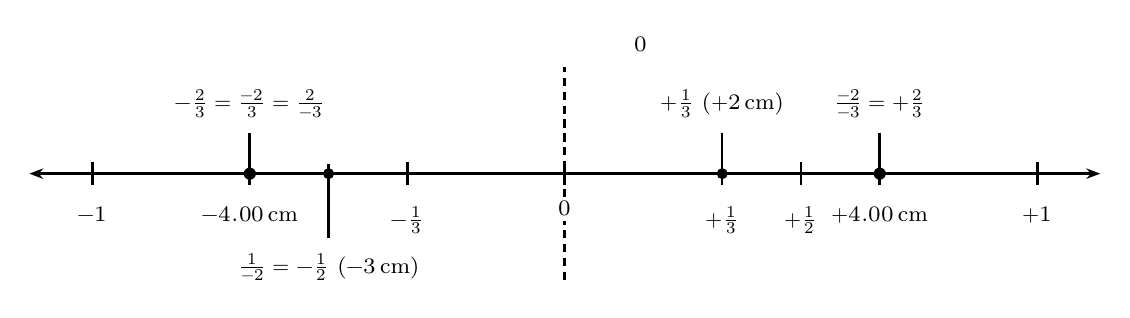
\begin{tikzpicture}[x=1cm, y=1cm, every node/.style={font=\footnotesize, text=black}]
    % បន្ទាត់បត់ត្រង់គល់ 0
    \draw[black, densely dashed, line width=1.0pt] (0,-1.35) -- (0,1.35);
    \node[above=2pt] at (0,1.35) {\textbf{បន្ទាត់បត់ឆ្លុះត្រង់គល់ $0$}};

    % អ័ក្សចំនួន [-6.8 cm, +6.8 cm]
    \draw[{Stealth[length=5pt]}-{Stealth[length=5pt]}, black, line width=1.2pt] (-6.80,0) -- (6.80,0);

    % ក្រិតសំខាន់ៗ៖ -1 (-6cm), -1/3 (-2cm), 0, +1/2 (+3cm), +1 (+6cm)
    \foreach \x/\lbl in {-6.00/-1, -2.00/-\frac{1}{3}, 3.00/+\frac{1}{2}, 6.00/+1} {
      \draw[black, line width=1.0pt] (\x,-0.15) -- (\x,0.15);
      \node[below=4pt] at (\x,-0.15) {$\lbl$};
    }
    \draw[black, line width=1.0pt] (0,-0.15) -- (0,0.15);
    \node[below=4pt, fill=white, inner sep=1.5pt] at (0,-0.15) {$0$};

    % POE 2A: -2/3 (-4.00 cm) និង +2/3 (+4.00 cm)
    \fill[black] (-4.00,0) circle (2.2pt);
    \draw[black, line width=0.95pt] (-4.00,-0.15) -- (-4.00,0.52);
    \node[above=2pt] at (-4.00,0.52) {$-\frac{2}{3}=\frac{-2}{3}=\frac{2}{-3}$};
    \node[below=4pt] at (-4.00,-0.15) {$-4.00\unit{cm}$};

    \fill[black] (4.00,0) circle (2.2pt);
    \draw[black, line width=0.95pt] (4.00,-0.15) -- (4.00,0.52);
    \node[above=2pt] at (4.00,0.52) {$\frac{-2}{-3}=+\frac{2}{3}$};
    \node[below=4pt] at (4.00,-0.15) {$+4.00\unit{cm}$};

    % POE 2B: 1/-2 (-3.00 cm) និង +1/3 (+2.00 cm)
    \fill[black] (-3.00,0) circle (2.0pt);
    \draw[black, line width=0.85pt] (-3.00,0.12) -- (-3.00,-0.82);
    \node[below=2pt] at (-3.00,-0.82) {$\frac{1}{-2}=-\frac{1}{2}$ ($-3\unit{cm}$)};

    \fill[black] (2.00,0) circle (2.0pt);
    \draw[black, line width=0.85pt] (2.00,-0.15) -- (2.00,0.52);
    \node[above=2pt] at (2.00,0.52) {$+\frac{1}{3}$ ($+2\unit{cm}$)};
    \node[below=4pt] at (2.00,-0.15) {$+\frac{1}{3}$};
  \end{tikzpicture}
  \end{center}
\end{tcolorbox}

\vspace{5pt}

% --- តារាងកត់ត្រាពិសោធន៍ POE 2A & 2B ---
{\renewcommand{\arraystretch}{1.42}
\begin{tabular}{|L{4.15cm}|L{4.15cm}|L{4.80cm}|L{4.55cm}|}
\hline
\rowcolor{headgray}
\textbf{ពិសោធន៍ \enbf{POE}} & \textbf{១. ទស្សន៍ទាយ (\enbf{Predict})} & \textbf{២. សង្កេតខ្នាត \enbf{1:1} (\enbf{Observe})} & \textbf{៣. ពន្យល់ក្បួន (\enbf{Explain})} \\
\hline
\textbf{\en{POE 2A}៖} តើ $-\dfrac{2}{3}$ ស្មើនឹង $\dfrac{-2}{-3}$ ដែរឬទេ? &
\chkbox\ ស្មើគ្នា \quad \chkbox\ មិនស្មើគ្នា &
$-\frac{2}{3}$ នៅចម្ងាយ \makebox[12mm]{\dotfill} ពី $0$ (ឆ្វេង)\par
$\frac{-2}{-3}$ នៅចម្ងាយ \makebox[12mm]{\dotfill} ពី $0$ (ស្ដាំ) &
ព្រោះ $(-)\div(-)=$ \makebox[12mm]{\dotfill}\par
ហាមចែកសញ្ញាដកទាំងលើទាំងក្រោម! \\
\hline
\textbf{\en{POE 2B}៖} ប្រៀបធៀប $\dfrac{1}{-2}$ និង $\dfrac{1}{3}$ ($b=-2<0$) &
បើគុណខ្វែងភ្លាម $1\cdot 3 > (-2)\cdot 1$ គេស្មានថា៖ $\frac{1}{-2}$ \makebox[8mm]{\dotfill} $\frac{1}{3}$ &
លើបន្ទាត់ចំនួនពិត៖\par
$\frac{1}{-2}$ ($-3\unit{cm}$) \makebox[8mm]{\dotfill} $\frac{1}{3}$ ($+2\unit{cm}$) &
មុនគុណខ្វែងវិសមភាព ត្រូវធ្វើឱ្យភាគបែង $b,d$ \makebox[14mm]{\dotfill} ជាមុនសិន! \\
\hline
\end{tabular}}

\clearpage

% ============================================================================
% ទំព័រទី ២៖ សម្ភារៈ E4 — កាតស៊ើបអង្កេត ៣ ជំហាន B&W + [tracing] (2-Up Cards)
% ============================================================================
\pagebanner{សម្ភារៈទី ២៖ កាតស៊ើបអង្កេត ៣ ជំហាន \enbf{B\&W + [tracing]} លើលំហាត់គំរូ \enbf{(2-Up)}}{ទំព័រ ២/៦ \en{-- E4 Elaborate}}

\newcommand{\DetectiveSheetE}[1]{%
\begin{tcolorbox}[
  enhanced, sharp corners, colback=white, colframe=black,
  boxrule=1.05pt, top=5pt, bottom=5pt, left=7pt, right=7pt
]
  {\muol\fontsize{9.5pt}{13.5pt}\selectfont កាតស៊ើបអង្កេត \enbf{E4} \enbf{(}សន្លឹកទី #1\enbf{)} — លំហាត់គំរូ \enbf{(}ទំព័រ ៥\enbf{)}}
  \hfill \textbf{ឈ្មោះដៃគូ៖} \makebox[45mm]{\dotfill}\\[3pt]
  \textbf{ប្រធាន៖} បញ្ជាក់ថា គូនៃចំនួនសនិទានខាងក្រោមស្មើគ្នា រួចសរសេរជា\textbf{ទម្រង់បង្រួមរួច}៖\par\vspace{3pt}
  {\renewcommand{\arraystretch}{1.32}\fontsize{9.0pt}{13.0pt}\selectfont
  \begin{tabular}{|L{2.55cm}|L{4.65cm}|L{5.20cm}|L{4.65cm}|}
  \hline
  \rowcolor{headgray}
  \textbf{គូចំនួនសនិទាន} & \textbf{ជំហានទី១៖ ព័ទ្ធរង្វង់សញ្ញាដក \cnum{3}} & \textbf{ជំហានទី២៖ អូសខ្វែង \enbf{[tracing]} \cnum{1}/\cnum{2}} & \textbf{ជំហានទី៣៖ ទម្រង់បង្រួមរួច \cnum{5}} \\
  \hline
  \textbf{ក.} $\dfrac{6}{-13}\; , \;\dfrac{-6}{13}$ &
  ព័ទ្ធរង្វង់សញ្ញាដកលើ $-13$ និង $-6$៖\par
  ភាគបែងវិជ្ជមានគឺ $b=13>0$ &
  $6 \times 13 = \makebox[14mm]{\dotfill}$\par
  $(-13)\times(-6) = \makebox[14mm]{\dotfill}$ &
  ស្មើគ្នាព្រោះ $ad=bc=\makebox[10mm]{\dotfill}$\par
  បង្រួមរួច៖ \makebox[22mm]{\dotfill} \\
  \hline
  \textbf{ខ.} $\dfrac{-25}{-35}\; , \;\dfrac{5}{7}$ &
  សញ្ញាដកទាំងពីរ៖ $(-)\div(-)=(+)$\par
  តួចែករួម $n = -5$ &
  $\dfrac{-25}{-35} = \dfrac{(-5)\times \makebox[7mm]{\dotfill}}{(-5)\times \makebox[7mm]{\dotfill}}$ &
  ស្មើនឹង $\dfrac{5}{7}$ តាមហេតុផល \cnum{2}\par
  បង្រួមរួច៖ \makebox[22mm]{\dotfill} \\
  \hline
  \textbf{គ.} $\dfrac{-15}{36}\; , \;\dfrac{20}{-48}$ &
  ព័ទ្ធរង្វង់ $-15$ និង $-48$៖\par
  រុញដក៖ $\dfrac{20}{-48} = \dfrac{-20}{48}$ &
  $(-15)\times(-48) = \makebox[14mm]{\dotfill}$\par
  $36 \times 20 = \makebox[14mm]{\dotfill}$ &
  សម្រួល $\dfrac{-15\div 3}{36\div 3} = \makebox[16mm]{\dotfill}$\par
  បង្រួមរួច៖ \makebox[22mm]{\dotfill} \\
  \hline
  \end{tabular}}\par\vspace{4pt}
  \begin{tcolorbox}[enhanced, sharp corners, colback=panelgray, colframe=black, boxrule=0.8pt, top=3pt, bottom=3pt, left=5pt, right=5pt]
    \fontsize{8.8pt}{12.5pt}\selectfont
    \textbf{សំណួរឆ្លុះបញ្ចាំង \en{EIA Looking-Back}៖} ក្នុងសំណួរ \textbf{(គ)} បើយើងសម្រួល $\dfrac{-15}{36}=\makebox[12mm]{\dotfill}$ និង $\dfrac{20}{-48}=\makebox[12mm]{\dotfill}$ មុន តើយើងចំណេញអ្វីខ្លះធៀបនឹងការគុណលេខធំ $36\times 20 = 720$? \textbf{ចម្លើយ៖} \makebox[68mm]{\dotfill}
  \end{tcolorbox}
\end{tcolorbox}}

\DetectiveSheetE{១}

\vspace{6pt}
\centerline{\scissors\dotfill\ \textbf{កាត់តាមបន្ទាត់ដាច់ៗនេះ ចែកជូនដៃគូសិស្ស ២ ក្រុម}\ \dotfill\scissors}
\vspace{6pt}

\DetectiveSheetE{២}

\clearpage

% ============================================================================
% ទំព័រទី ៣៖ សម្ភារៈ E5 — សន្លឹក Relay ក្រុម ៣ តួនាទី + អ្នកប្រមាញ់តម្លៃ -5
% ============================================================================
\pagebanner{សម្ភារៈទី ៣៖ សន្លឹក \enbf{Relay} ក្រុម ៣ តួនាទី \enbf{(Pause-Review)} — ប្រតិបត្តិ \enbf{\&} លំហាត់ ១}{ទំព័រ ៣/៦ \en{-- E5 Evaluate}}

\begin{tcolorbox}[
  enhanced, sharp corners, colback=panelgray, colframe=black,
  boxrule=1.0pt, top=4pt, bottom=4pt, left=7pt, right=7pt
]
  \textbf{ក្រុមទី៖} \makebox[15mm]{\dotfill} \quad
  \textbf{តួនាទីទី១ (រៀបសញ្ញា \cnum{3})៖} \makebox[28mm]{\dotfill} \quad
  \textbf{ទី២ (ផ្ទៀងសមមូល \cnum{1}/\cnum{2})៖} \makebox[28mm]{\dotfill} \quad
  \textbf{ទី៣ (បង្រួមរួច \cnum{5})៖} \makebox[28mm]{\dotfill}\\[2pt]
  \textbf{អ្នកត្រួតពិនិត្យ \en{Pause-Review} (សមាជិកទី៤)៖} \makebox[35mm]{\dotfill} — ផ្ទៀងថាគ្រប់ចម្លើយបង្រួមរួចមានភាគបែងវិជ្ជមាន ($b>0$) និងដាក់លេខ \cnum{1}--\cnum{5} ត្រឹមត្រូវ!
\end{tcolorbox}

\vspace{5pt}

{\muol\fontsize{10pt}{14.5pt}\selectfont ភារកិច្ចទី ១៖ ប្រតិបត្តិ \enbf{(}សៀវភៅសិក្សាគោល ទំព័រ ៥\enbf{)} — បញ្ជាក់ភាពស្មើគ្នា និងសរសេរជាទម្រង់បង្រួមរួច}
\vspace{3pt}

{\renewcommand{\arraystretch}{1.48}
\begin{tabular}{|L{3.10cm}|L{4.80cm}|L{5.30cm}|L{4.50cm}|}
\hline
\rowcolor{headgray}
\textbf{លំហាត់ប្រតិបត្តិ} & \textbf{តួនាទីទី១៖ រៀបសញ្ញា \cnum{3}} & \textbf{តួនាទីទី២៖ បញ្ជាក់ស្មើគ្នា \cnum{1}/\cnum{2}} & \textbf{តួនាទីទី៣៖ ទម្រង់បង្រួមរួច \cnum{5}} \\
\hline
\textbf{ក.} $\dfrac{16}{-30}\; , \;\dfrac{-8}{15}$ &
រុញសញ្ញាដកឡើងភាគយក៖\par
$\dfrac{16}{-30} = \makebox[24mm]{\dotfill}$\par
ហេតុផល៖ លេខ \makebox[10mm]{\dotfill} &
អូសខ្វែង \en{[tracing]}៖\par
$16 \times 15 = \makebox[18mm]{\dotfill}$\par
$(-30)\times(-8) = \makebox[18mm]{\dotfill}$ &
សម្រួលនឹង $\text{តួចែករួមធំបំផុត}=\makebox[8mm]{\dotfill}$៖\par
ទម្រង់បង្រួមរួចគឺ៖ \makebox[20mm]{\dotfill}\par
ផ្ទៀង $b>0$៖ \chkbox\ ត្រឹមត្រូវ \\
\hline
\textbf{ខ.} $\dfrac{-15}{-35}\; , \;\dfrac{21}{49}$ &
សញ្ញាដកពីរជាន់ $(-)\div(-)$៖\par
$\dfrac{-15}{-35} = \makebox[24mm]{\dotfill}$\par
ហេតុផល៖ លេខ \makebox[10mm]{\dotfill} &
សម្រួលប្រភាគទាំងពីរ ឬគុណខ្វែង៖\par
$\dfrac{15\div 5}{35\div 5} = \makebox[14mm]{\dotfill}$ \; ; \;
$\dfrac{21\div 7}{49\div 7} = \makebox[14mm]{\dotfill}$ &
ប្រភាគទាំងពីរស្មើគ្នា!\par
ទម្រង់បង្រួមរួចគឺ៖ \makebox[20mm]{\dotfill}\par
ផ្ទៀង $b>0$៖ \chkbox\ ត្រឹមត្រូវ \\
\hline
\end{tabular}}

\vspace{7pt}

{\muol\fontsize{10pt}{14.5pt}\selectfont ភារកិច្ចទី ២៖ អ្នកប្រមាញ់តម្លៃ \enbf{-5} \enbf{(}លំហាត់ ១ ទំព័រ ១១\enbf{)}}
\vspace{3pt}

\begin{tcolorbox}[
  enhanced, sharp corners, colback=white, colframe=black,
  boxrule=1.0pt, top=5pt, bottom=5pt, left=7pt, right=7pt
]
  \textbf{ប្រធាន (ទំព័រ ១១)៖} ក្នុងចំណោមចំនួនខាងក្រោម តើចំនួនណាខ្លះដែលស្មើ $-5$ ? ចូរគូសធីក \chkbox\ លើប្រអប់ស្មើ $-5$ និងសរសេរតម្លៃពិត ($-5$ ឬ $+5$)៖\\[5pt]
  {\renewcommand{\arraystretch}{1.45}
  \begin{tabular}{|C{2.25cm}|C{2.25cm}|C{2.25cm}|C{2.25cm}|C{2.25cm}|C{2.25cm}|C{2.35cm}|}
  \hline
  \rowcolor{headgray}
  $\dfrac{-5}{1}$ & $\dfrac{5}{1}$ & $\dfrac{5}{-1}$ & $-\dfrac{5}{1}$ & $\dfrac{-5}{-1}$ & $-\dfrac{-5}{1}$ & $-\dfrac{-5}{-1}$ \\[4pt]
  \hline
  តម្លៃ៖ \makebox[10mm]{\dotfill} & តម្លៃ៖ \makebox[10mm]{\dotfill} & តម្លៃ៖ \makebox[10mm]{\dotfill} & តម្លៃ៖ \makebox[10mm]{\dotfill} & តម្លៃ៖ \makebox[10mm]{\dotfill} & តម្លៃ៖ \makebox[10mm]{\dotfill} & តម្លៃ៖ \makebox[10mm]{\dotfill} \\
  \chkbox\ ស្មើ $-5$ & \chkbox\ ស្មើ $-5$ & \chkbox\ ស្មើ $-5$ & \chkbox\ ស្មើ $-5$ & \chkbox\ ស្មើ $-5$ & \chkbox\ ស្មើ $-5$ & \chkbox\ ស្មើ $-5$ \\
  \hline
  \end{tabular}}\\[5pt]
  \textbf{ក្បួនសម្គាល់រហ័សរបស់ក្រុម៖} កន្សោមដែលមានសញ្ញាដកចំនួន \makebox[20mm]{\dotfill} (គូ/សេស) ស្មើ $-5$ សរុបមាន \makebox[10mm]{\dotfill} ចំនួន។
\end{tcolorbox}

\vspace{6pt}

\begin{tcolorbox}[
  enhanced, sharp corners, colback=panelgray, colframe=black,
  boxrule=1.0pt, top=5pt, bottom=5pt, left=7pt, right=7pt
]
  {\muol\fontsize{9.6pt}{13.5pt}\selectfont ភារកិច្ចទី ៣៖ បិទបញ្ចប់បេសកកម្ម \enbf{E1} — ស្លាកកម្ពស់ទឹកក្រោមស្ពានកំពង់ស្វាយ}\\[3pt]
  ក្នុងចំណោមស្លាក $-\dfrac{6}{13}\unit{m},\; \dfrac{-6}{13}\unit{m},\; \dfrac{6}{-13}\unit{m}$ និង $\dfrac{-6}{-13}\unit{m}$៖\par\vspace{2pt}
  $\bullet$ ស្លាកបង្ហាញជម្រៅដូចគ្នាក្រោមគំនូស $0\unit{m}$ គឺ៖ \makebox[65mm]{\dotfill} (តាមហេតុផលលេខ \makebox[10mm]{\dotfill})\par\vspace{2pt}
  $\bullet$ ស្លាកដែលច្រឡំទៅលើគំនូស $0\unit{m}$ គឺ៖ \makebox[35mm]{\dotfill} ព្រោះវាស្មើនឹង \makebox[25mm]{\dotfill} ។
\end{tcolorbox}

\clearpage

% ============================================================================
% ទំព័រទី ៤៖ សម្ភារៈទី ៤ — ផ្ទាំងធនាគារហេតុផល ①–⑤ (Classroom Warrant Poster)
% ============================================================================
\pagebanner{សម្ភារៈទី ៤៖ ផ្ទាំងធនាគារហេតុផល \enbf{Warrant Bank (1--5)} សម្រាប់បិទលើក្ដារខៀន \enbf{/} តុក្រុម}{ទំព័រ ៤/៦ \en{-- E3--E5 Poster}}

\begin{center}
{\muol\fontsize{13pt}{18pt}\selectfont ធនាគារហេតុផលគណិតវិទ្យា — ២.៣ លក្ខណៈនៃចំនួនសនិទាន}\\[3pt]
{\fontsize{10pt}{14pt}\selectfont រចនាសម្ព័ន្ធគំនិត \en{Hub-and-Spoke}៖ គ្រប់ការសម្រាយបញ្ជាក់ត្រូវសរសេរលេខសំអាង \cnum{1}--\cnum{5} ជានិច្ច!}
\end{center}

\vspace{4pt}

\begin{center}
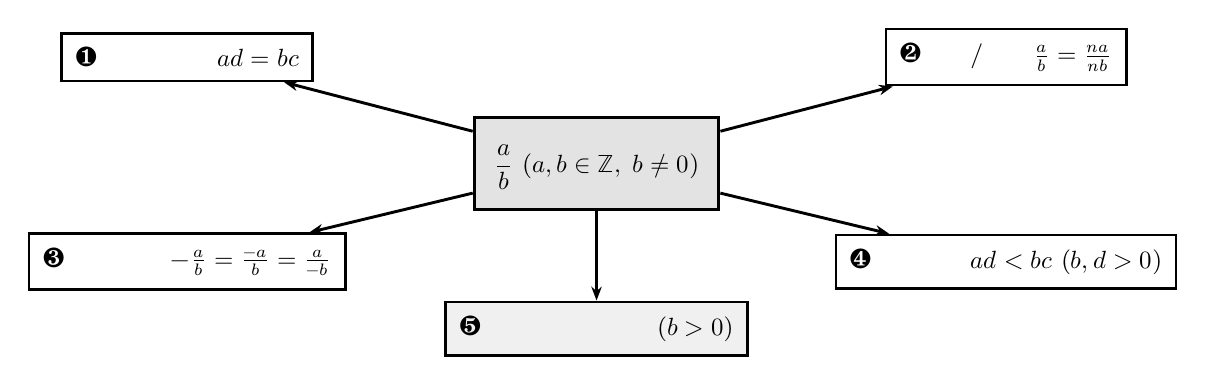
\begin{tikzpicture}[x=1cm, y=1cm, every node/.style={font=\small, text=black}]
  \node[draw=black, line width=1.3pt, fill=gray!22, inner sep=7pt, align=center] (hub) at (0,0)
    {\textbf{ស្នូលចំនួនសនិទាន}\\[2pt] $\dfrac{a}{b}$ ($a,b\in\mathbb{Z},\; b\neq 0$)};
  \node[draw=black, line width=1.0pt, fill=white, inner sep=5pt] (s1) at (-5.2,1.35) {\cnum{1}\;សមមូលផលគុណខ្វែង $ad=bc$};
  \node[draw=black, line width=1.0pt, fill=white, inner sep=5pt] (s2) at (5.2,1.35) {\cnum{2}\;ពង្រីក/សម្រួល $\frac{a}{b}=\frac{na}{nb}$};
  \node[draw=black, line width=1.0pt, fill=white, inner sep=5pt] (s3) at (-5.2,-1.25) {\cnum{3}\;ទីតាំងសញ្ញាដក $-\frac{a}{b}=\frac{-a}{b}=\frac{a}{-b}$};
  \node[draw=black, line width=1.0pt, fill=white, inner sep=5pt] (s4) at (5.2,-1.25) {\cnum{4}\;វិសមភាពខ្វែង $ad<bc$ ($b,d>0$)};
  \node[draw=black, line width=1.05pt, fill=gray!12, inner sep=5pt] (s5) at (0,-2.10) {\cnum{5}\;ទម្រង់បង្រួមរួចស្ដង់ដារ ($b>0$)};

  \draw[black, line width=1.05pt, -{Stealth[length=5pt]}] (hub) -- (s1);
  \draw[black, line width=1.05pt, -{Stealth[length=5pt]}] (hub) -- (s2);
  \draw[black, line width=1.05pt, -{Stealth[length=5pt]}] (hub) -- (s3);
  \draw[black, line width=1.05pt, -{Stealth[length=5pt]}] (hub) -- (s4);
  \draw[black, line width=1.05pt, -{Stealth[length=5pt]}] (hub) -- (s5);
\end{tikzpicture}
\end{center}

\vspace{6pt}

\newcommand{\warrantcard}[3]{%
  \begin{tcolorbox}[
    enhanced, sharp corners, colback=white, colframe=black,
    boxrule=1.1pt, left=8pt, right=8pt, top=5pt, bottom=5pt, after skip=6pt
  ]
    {\fontsize{11pt}{15.5pt}\selectfont\textbf{#1 — #2}}\\[3pt]
    {\fontsize{10.2pt}{15pt}\selectfont #3}
  \end{tcolorbox}%
}

\warrantcard{\cnum{1}}{សមមូលផលគុណខ្វែង (លក្ខណៈទី១ ទំព័រ ៥)}{%
  តាង $\dfrac{a}{b}$ និង $\dfrac{c}{d}$ ជាពីរចំនួនសនិទាន ($b\neq 0,\; d\neq 0$) នោះ៖
  $\qquad \dfrac{a}{b} = \dfrac{c}{d} \iff ad = bc$ ។}

\warrantcard{\cnum{2}}{ការពង្រីក និងសម្រួលប្រភាគ (លក្ខណៈទី២ ទំព័រ ៥)}{%
  តាង $\dfrac{a}{b}$ ជាចំនួនសនិទាន និង $n\in\mathbb{Z},\; n\neq 0$ នោះ៖
  $\qquad \dfrac{a}{b} = \dfrac{na}{nb} \quad \text{និង} \quad \dfrac{na}{nb} = \dfrac{a}{b}$ ។}

\warrantcard{\cnum{3}}{ក្បួនទីតាំងសញ្ញាដកទាំង ៣ និងវិបាកសញ្ញាដកពីរជាន់ (លក្ខណៈទី៣ ទំព័រ ៥)}{%
  $-\dfrac{a}{b} = \dfrac{-a}{b} = \dfrac{a}{-b}$ \quad (សញ្ញាដក \textbf{១} ៖ អវិជ្ជមានដូចគ្នា) \qquad $\Big|$ \qquad
  $\dfrac{-a}{-b} = +\dfrac{a}{b}$ \quad (សញ្ញាដក \textbf{២} ៖ វិជ្ជមាន!)។}

\warrantcard{\cnum{4}}{វិសមភាពផលគុណខ្វែងក្រោមលក្ខខណ្ឌភាគបែងវិជ្ជមាន (លក្ខណៈទី៤ ទំព័រ ៥)}{%
  ចំពោះតែ \textbf{$b > 0$ និង $d > 0$} ប៉ុណ្ណោះ៖ $\dfrac{a}{b} < \dfrac{c}{d} \iff ad < bc$ ។ \textbf{ប្រយ័ត្ន៖} បើភាគបែងអវិជ្ជមាន ត្រូវប្រើ \cnum{3} ជាមុន!}

\warrantcard{\cnum{5}}{និយមន័យទម្រង់បង្រួមរួចស្ដង់ដារ (\en{Canonical Irreducible Form})}{%
  ប្រភាគ $\dfrac{a}{b}$ ជាទម្រង់បង្រួមរួចស្ដង់ដារ លុះត្រាតែ៖ \textbf{(១) ភាគបែងវិជ្ជមាន $b > 0$} និង \textbf{(២) $\text{តួចែករួមធំបំផុត }(|a|,b) = 1$} ។}

\clearpage

% ============================================================================
% ទំព័រទី ៥៖ សម្ភារៈ E5 — បណ្ណស្ទង់មតិរហ័ស Exit Foils A–D + កូនសោវិនិច្ឆ័យគ្រូ
% ============================================================================
\pagebanner{សម្ភារៈទី ៥៖ បណ្ណលើកឆ្លើយរហ័ស \enbf{Exit Foils (A--D)} \enbf{\&} កូនសោវិនិច្ឆ័យកំហុសសម្រាប់គ្រូ}{ទំព័រ ៥/៦ \en{-- E5 Diagnostic}}

{\textbf{\scissors\ ផ្នែកកាត់ទី១ — បណ្ណលើកឆ្លើយរហ័ស \en{A, B, C, D} (កាត់ចែកសិស្សម្នាក់ ១ ឈុត លើកឆ្លើយព្រមគ្នាក្នុង ៩០ វិនាទី)៖}}
\vspace{4pt}

\noindent
\begin{tabular}{|C{4.35cm}|C{4.35cm}|C{4.35cm}|C{4.35cm}|}
\hline
\rule{0pt}{1.75cm}{\TimesEn\bfseries\fontsize{38pt}{40pt}\selectfont A}\par\vspace{6pt}
{\fontsize{9pt}{12pt}\selectfont បណ្ណជម្រើស \enbf{A}}\par\vspace{4pt} &
\rule{0pt}{1.75cm}{\TimesEn\bfseries\fontsize{38pt}{40pt}\selectfont B}\par\vspace{6pt}
{\fontsize{9pt}{12pt}\selectfont បណ្ណជម្រើស \enbf{B}}\par\vspace{4pt} &
\rule{0pt}{1.75cm}{\TimesEn\bfseries\fontsize{38pt}{40pt}\selectfont C}\par\vspace{6pt}
{\fontsize{9pt}{12pt}\selectfont បណ្ណជម្រើស \enbf{C}}\par\vspace{4pt} &
\rule{0pt}{1.75cm}{\TimesEn\bfseries\fontsize{38pt}{40pt}\selectfont D}\par\vspace{6pt}
{\fontsize{9pt}{12pt}\selectfont បណ្ណជម្រើស \enbf{D}}\par\vspace{4pt} \\
\hline
\end{tabular}

\vspace{8pt}
\centerline{\scissors\dotfill\ \textbf{ផ្នែកទី២៖ សំណួរស្ទង់មតិរហ័សលើក្ដារខៀន (៦០--៩០ វិនាទី)}\ \dotfill\scissors}
\vspace{6pt}

\begin{tcolorbox}[
  enhanced, sharp corners, colback=white, colframe=black,
  boxrule=1.05pt, top=6pt, bottom=6pt, left=8pt, right=8pt
]
  \textbf{សំណួរទី ១៖} តើមួយណាជា \textbf{ទម្រង់បង្រួមរួចស្ដង់ដារ} នៃចំនួនសនិទាន $\dfrac{18}{-42}$ ?\\[4pt]
  \hspace*{0.5cm}\enbf{A.}\; $\dfrac{3}{-7}$ \hspace{2.4cm}
  \enbf{B.}\; $\dfrac{-3}{-7}$ \hspace{2.4cm}
  \enbf{C.}\; $\dfrac{-3}{7}$ \hspace{2.4cm}
  \enbf{D.}\; $\dfrac{-9}{21}$\\[8pt]
  \textbf{សំណួរទី ២៖} ដើម្បីប្រៀបធៀប $\dfrac{3}{-4}$ និង $\dfrac{-5}{7}$ ដោយប្រើផលគុណខ្វែងតាមលក្ខណៈទី៤ តើជំហានទី១ ដែលត្រឹមត្រូវគឺមួយណា?\\[4pt]
  \hspace*{0.5cm}\enbf{A.}\; គុណខ្វែង $3\times 7 > (-4)\times(-5)$ ភ្លាមៗ \hspace{1.75cm}
  \enbf{B.}\; ប្ដូរ $\dfrac{3}{-4} = \dfrac{-3}{4}$ ឱ្យភាគបែងវិជ្ជមានជាមុន\\[3pt]
  \hspace*{0.5cm}\enbf{C.}\; ប្ដូរ $\dfrac{3}{-4} = \dfrac{-3}{-4}$ ដើម្បីឱ្យដកទាំងលើទាំងក្រោម \hspace{0.95cm}
  \enbf{D.}\; លុបសញ្ញាដកចោល រួចប្រៀបធៀប $\dfrac{3}{4}$ និង $\dfrac{5}{7}$
\end{tcolorbox}

\vspace{8pt}

{\muol\fontsize{10pt}{14.5pt}\selectfont ផ្នែកទី ៣៖ កូនសោវិនិច្ឆ័យកំហុសភ្លាមៗសម្រាប់គ្រូបង្រៀន \enbf{(Teacher Diagnostic Key)}}
\vspace{3pt}

{\renewcommand{\arraystretch}{1.38}
\begin{tabular}{|C{1.65cm}|C{1.65cm}|L{6.80cm}|L{7.60cm}|}
\hline
\rowcolor{headgray}
\textbf{សំណួរ} & \textbf{បណ្ណ} & \textbf{ការវិនិច្ឆ័យការគិតរបស់សិស្ស} & \textbf{អន្តរាគមន៍កែតម្រូវរហ័ស ១៥ វិនាទី} \\
\hline
ទី ១ & \enbf{A} ($\frac{3}{-7}$) & សម្រួលនឹង $6$ ត្រូវ តែទុកភាគបែងអវិជ្ជមាន ($b=-7<0$)។ & ចង្អុលហេតុផល \cnum{5}៖ រុញដកឡើងលើតាម \cnum{3} បាន $\frac{-3}{7}$។ \\
\hline
ទី ១ & \enbf{B} ($\frac{-3}{-7}$) & ចែកសញ្ញាដកទៅទាំងភាគយកនិងភាគបែង (ក្លាយជា $+\frac{3}{7}$)! & រំលឹកបន្ទាត់ចំនួនឆ្លុះ \en{POE 2A}៖ $(-)\div(-)=(+)$ ខុសសញ្ញាដើម។ \\
\hline
ទី ១ & \textbf{\enbf{C} ($\frac{-3}{7}$)} & \textbf{ចម្លើយត្រឹមត្រូវ ១០០\%} ($b=7>0$ និង $\gcd(3,7)=1$)។ & សរសើរ និងឱ្យសិស្សបញ្ជាក់លេខសំអាង \cnum{2}+\cnum{3}+\cnum{5}។ \\
\hline
ទី ១ & \enbf{D} ($\frac{-9}{21}$) & រុញសញ្ញាដកត្រូវ តែសម្រួលនឹង $2$ ប៉ុណ្ណោះ (នៅសល់តួចែករួម $3$)។ & រំលឹកឱ្យចែកនឹង $\text{តួចែករួមធំបំផុត }(18,42)=6$។ \\
\hline
ទី ២ & \enbf{A / C / D} & \enbf{A}: អន្ទាក់គុណខ្វែងទាំង $b=-4<0$ (\en{Çetin, 2022}); \enbf{C}: ដកពីរជាន់; \enbf{D}: បោះបង់សញ្ញា។ & \textbf{ចម្លើយត្រឹមត្រូវគឺ \enbf{B}}៖ ប្ដូរ $\frac{3}{-4}=\frac{-3}{4}$ ($b=4>0, d=7>0$) រួចគុណខ្វែង $(-3)\times 7 = -21 < 4\times(-5) = -20$។ \\
\hline
\end{tabular}}

\clearpage

% ============================================================================
% ទំព័រទី ៦៖ សម្ភារៈជំហានទី៥ — ប័ណ្ណកិច្ចការផ្ទះកាត់ចែក (2-Up Verbatim Slips)
% ============================================================================
\pagebanner{សម្ភារៈទី ៦៖ ប័ណ្ណកិច្ចការផ្ទះកាត់ចែកសិស្ស \enbf{(2-Up)} — ត្រូវគ្នាពាក្យ\enbf{-}ទល់\enbf{-}ពាក្យនឹង \enbf{LS\_Plan}}{ទំព័រ ៦/៦ \en{-- Step 5 Homework}}

\newcommand{\HomeworkSlipRAT}[1]{%
\begin{tcolorbox}[
  enhanced, sharp corners, colback=white, colframe=black,
  boxrule=1.05pt, top=5pt, bottom=5pt, left=8pt, right=8pt
]
  {\muol\fontsize{9.6pt}{14pt}\selectfont ប័ណ្ណកិច្ចការផ្ទះ \enbf{(}សន្លឹកទី #1\enbf{)} — មេរៀនទី១៖ ២.៣ លក្ខណៈនៃចំនួនសនិទាន}\\[2pt]
  \textbf{ឈ្មោះសិស្ស៖} \makebox[48mm]{\dotfill} \quad \textbf{ថ្នាក់ទី៨៖} \makebox[14mm]{\dotfill} \quad \textbf{កាលបរិច្ឆេទ៖} ១៦ វិច្ឆិកា ២០២៦\\[4pt]
  \textbf{ក.} បញ្ជាក់ថាគូចំនួនសនិទានខាងក្រោមស្មើគ្នា រួចសរសេរជាទម្រង់បង្រួមរួច (បញ្ជាក់លេខហេតុផល \cnum{1}--\cnum{5})៖\\[3pt]
  \hspace*{0.3cm}១) $\dfrac{-18}{45}\; , \;\dfrac{14}{-35}$ \dotfill\\[4pt]
  \hspace*{0.75cm}ទម្រង់បង្រួមរួចគឺ៖ \makebox[35mm]{\dotfill} \quad ហេតុផលប្រើប្រាស់៖ \makebox[35mm]{\dotfill}\\[5pt]
  \hspace*{0.3cm}២) $\dfrac{-24}{-56}\; , \;\dfrac{15}{35}$ \dotfill\\[4pt]
  \hspace*{0.75cm}ទម្រង់បង្រួមរួចគឺ៖ \makebox[35mm]{\dotfill} \quad ហេតុផលប្រើប្រាស់៖ \makebox[35mm]{\dotfill}\\[6pt]
  \textbf{ខ.} ១) ក្នុងចំណោម $-\dfrac{7}{1},\; \dfrac{-7}{-1},\; \dfrac{7}{-1},\; -\dfrac{-7}{1},\; -\dfrac{-7}{-1}$ តើចំនួនណាខ្លះស្មើ $-7$ ?\\[3pt]
  \hspace*{0.75cm}\textbf{ចម្លើយ៖} ចំនួនដែលស្មើ $-7$ គឺ \dotfill\\[5pt]
  \hspace*{0.3cm}២) ប្រៀបធៀប $\dfrac{5}{-8}$ និង $\dfrac{-3}{5}$ ដោយប្រើលក្ខណៈទី៣ និងទី៤ (\cnum{3}$\to$\cnum{4})៖\\[3pt]
  \hspace*{0.75cm}ជំហានទី១ (ប្ដូរភាគបែងវិជ្ជមាន \cnum{3})៖ $\dfrac{5}{-8} = \makebox[22mm]{\dotfill}$ \quad ជំហានទី២ (ផលគុណខ្វែង \cnum{4})៖ \dotfill\\[4pt]
  \hspace*{0.75cm}\textbf{សន្និដ្ឋាន៖} $\dfrac{5}{-8}$ \makebox[12mm]{\dotfill} $\dfrac{-3}{5}$ \qquad
  {\fontsize{8.5pt}{11.5pt}\selectfont\textit{(អានមុន៖ ៣.១ ប្រមាណវិធីបូកនៃចំនួនសនិទាន ទំព័រ ៥)}}
\end{tcolorbox}}

\HomeworkSlipRAT{១}

\vspace{8pt}
\centerline{\scissors\dotfill\ \textbf{កាត់តាមបន្ទាត់ដាច់ៗនេះ ចែកសិស្ស ២ នាក់ក្នុង ១ សន្លឹក \en{A4}}\ \dotfill\scissors}
\vspace{8pt}

\HomeworkSlipRAT{២}

\end{document}
